\section{Characteristics of Mainstream Playlists}
We analyzed the difference between playlists that contain an above-average amount of mainstream tracks and playlists that contain mostly uncommon tracks. For this we first had to establish a measurement from which we can identify a playlist as mainstream. As previously described we have calculated the most common tracks. We determined an arbitrary but reasonable border, which is to contain at least three of the top 50 common tracks to count as a mainstream playlist. To obtain the same group sizes between mainstream and uncommon playlists, we sampled from the larger one (uncommon playlist). We then looked for differences between the groups and found that playlists with popular tracks have less unique artists than playlists with unpopular tracks. 

\begin{figure}[ht]
    \centering
    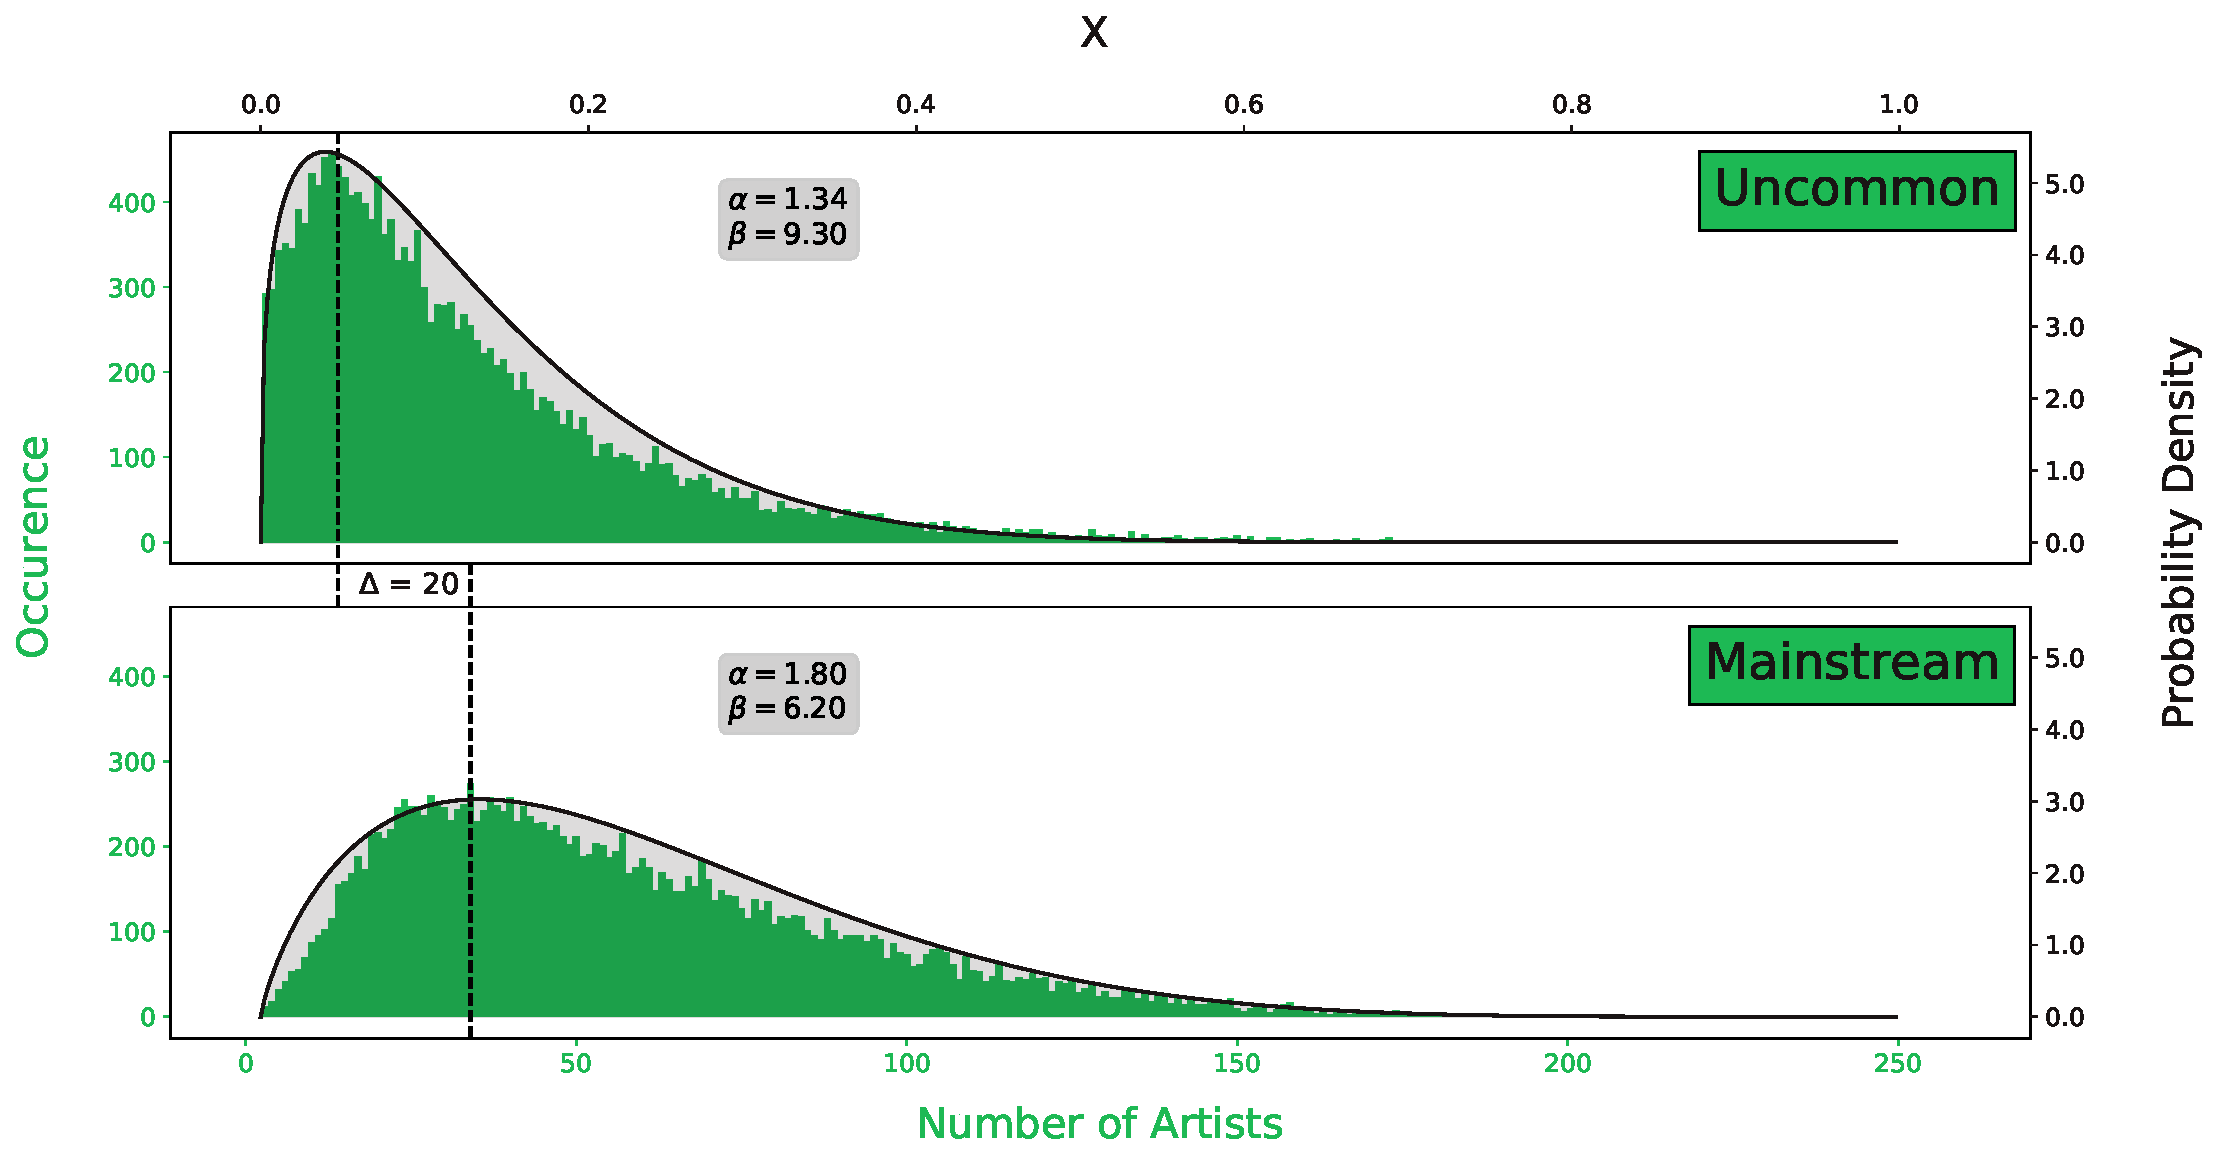
\includegraphics[width=\textwidth]{fig/pop_unpop_artist.pdf}
    \caption{Histogram of Number of Artists (\textcolor{spotifygreen}{---}) with fitted Beta distribution (\textcolor{black}{---}) for uncommon and mainstream playlists}
    \label{fig:pop_unppo_artist}
\end{figure}

To show this we plotted the number of artists against its occurrence for both groups. Just by looking at the mode (Uncommon=14; Mainstream=34) we can see that there is a difference but to further underlie our finding we fitted a beta distribution to the data. The input values of a beta distribution are between 0 and 1. Since the playlists in the dataset are constrained to have at least three but no more than 250 artists, also the data has limits on both sides. The probability density of both beta distributions is shifted to the lower border. We can see that the beta distribution of uncommon playlists has nearly all of its mass around the mode, while the mass of the beta distribution of mainstream playlists is much more spread.

We also thought of metric that can directly measure the popularity of a playlist, which is the number of followers of a playlist. The playlists are constrained to have at least one follower and more than 90\% of the playlist have three or less. This is why we decided to not split the data into the binary groups, popular and unpopular. Nevertheless, we found that the more follower a playlist has, the more likely it is for the playlist to have a description.

\begin{figure}[ht]
    \centering
    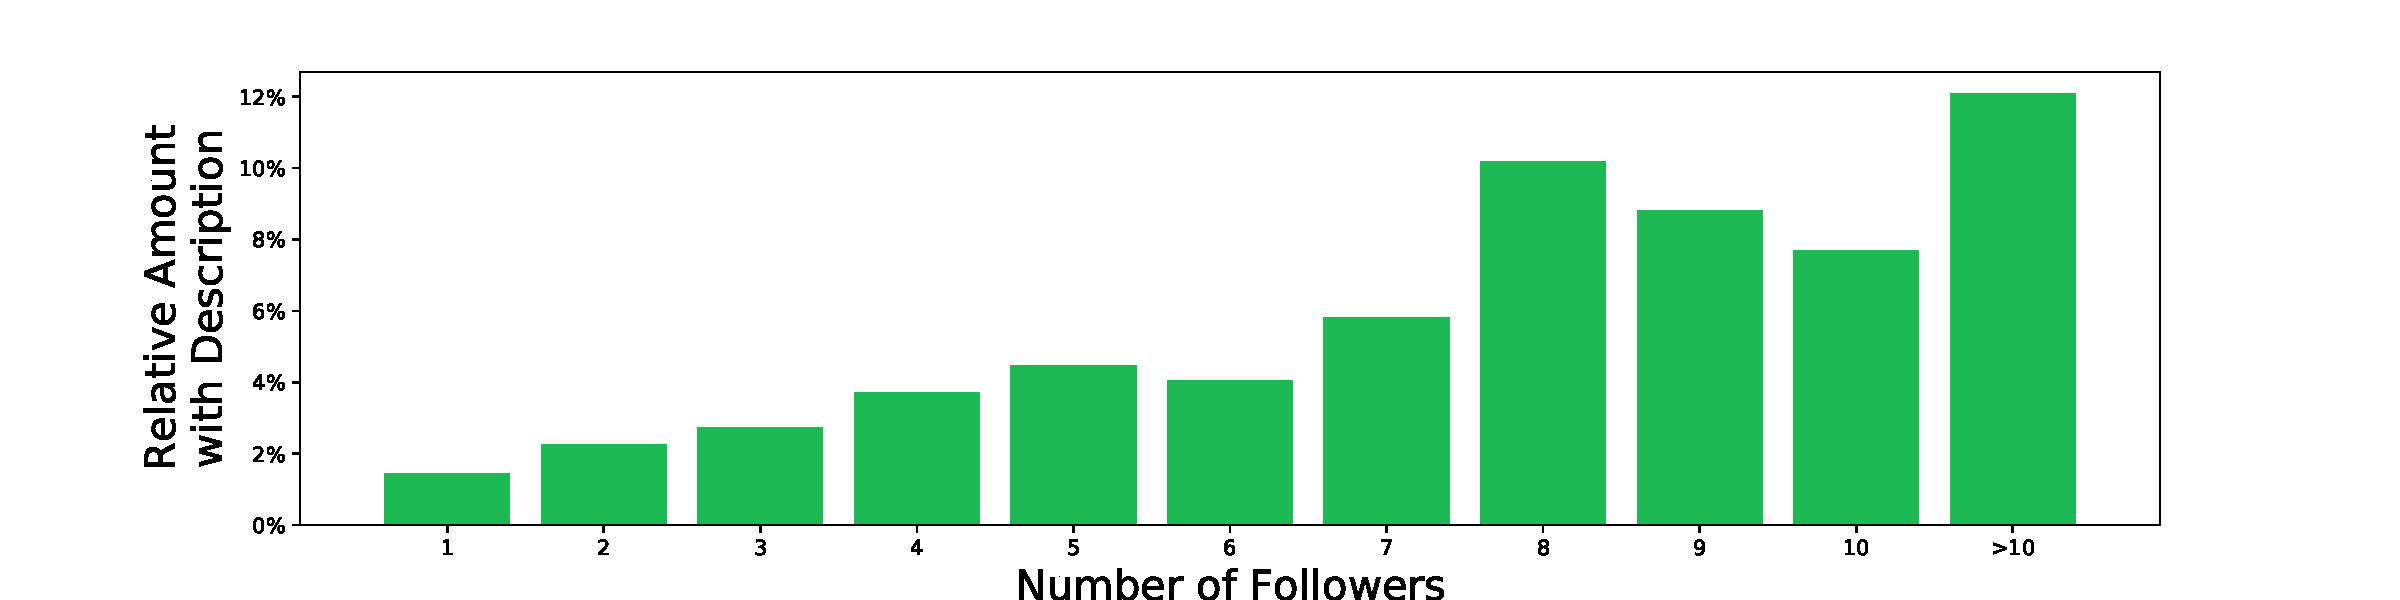
\includegraphics[width=\textwidth]{fig/followers_to_description.pdf}
    \caption{Bar plot of number of followers to relative amount with description}
    \label{fig:followers_to_description}
\end{figure}

We grouped the playlists by their follower number and counted the ones that have been given a description. Because the groups heavily differ in size, we calculated the relative amount. As mentioned, the data pool for playlists with higher follower numbers gets very small. That is why we put all playlists with more than ten followers into a single group.